% !TeX spellcheck = pt_BR
\documentclass{beamer}
\usepackage[brazilian]{babel}
\usepackage[utf8]{inputenc}
%\usepackage{pgfpages}
\usepackage{amsmath}
\usetheme{CambridgeUS}
\usecolortheme{seahorse}

%usar a usepackage pgfpages com as notas de segunda tela
%\setbeameroption{show notes on second screen}
%\usepackage{hyperref}


%Sonar, Relógio e Lentes Acústicas
\title[Detector de Objetos]{Detecção de Objetos usando Redes Neurais}
\subtitle{Interface Web}
\author{Rafael Mendes Campello}

\date{11 de Maio de 2019}
%\subject{Tecnologia dos Materiais}

%\titlegraphic{
%	\includegraphics[scale=0.15]{Images/ufpe_gs.png}
%}

%\AtBeginSection[]{
%	\begin{frame}
%	\tableofcontents[currentsection]
%	\end{frame}
%}

\setbeamertemplate{itemize items}[ball]
\setbeamertemplate{caption}{\raggedright\insertcaption\par}

\definecolor{bistre}{rgb}{0.24, 0.17, 0.12}
\newcommand{\btVFill}{\vskip0pt plus 1filll}
\newcommand{\frameref}[1]{\btVFill \color{bistre}\scriptsize #1}

\begin{document}
	\section{Capa}
	\begin{frame}
		\titlepage

%		\note{ver o que as apresentações iniciais vão fazer aqui e fazer igual}
	\end{frame}

	\section{Rede Neurais}
	\subsection{Overview}
	\begin{frame}
		\frametitle{Overview}
		
		A linguagem de programação escolhida foi Python.
		
		\begin{itemize}
			\item O problema de detectar objetos em imagens era um problema difícil até pouco tempo atrás.
			\item Hoje, com o crescimento e exploração das aplicações de Redes Neurais, existem diversas redes disponíveis na internet já pré-treinadas ou com estrutura pronta para treino.
			\item Alguns exemplos de redes facilmente encontradas que realizam esta tarefa são:
			\begin{itemize}
				\item Yolo (darknet)
				\item ResNet50
				\item RetinaNet
			\end{itemize}
		\end{itemize}
	\end{frame}
	
	\subsection{ResNet50}
	\begin{frame}
		\frametitle{ResNet50}
		Foi escolhida a ResNet50.
		
		\begin{itemize}
			\item Rede Neural clássica para tarefas de Visão Computacional.
			\item Rede Residual de 50 camadas.
			\item Implementação pode ser feita com TensorFlow/Keras.
		\end{itemize}
	\end{frame}
	
	
	
	\subsection{Desempenho}
	
	\begin{frame}
	\frametitle{Desempenho}
			
		Inicialmente, foi feito um script simples para receber uma imagem e detectar objetos/animais/pessoas.
		
		
		\begin{figure}
			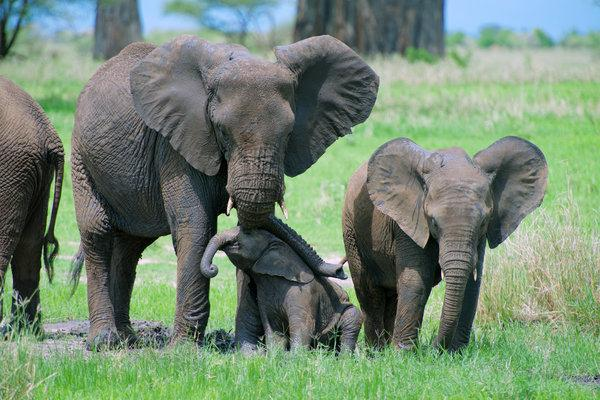
\includegraphics[scale=0.25]{../media/Elephant}
			\hspace{0.6cm}
			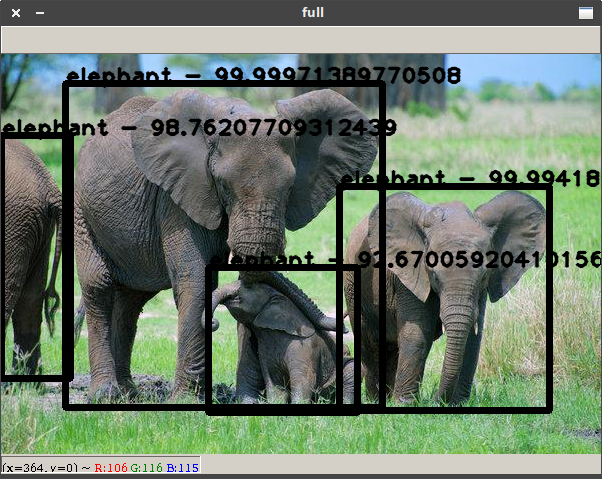
\includegraphics[scale=0.25]{Imgs/elefantes_classificados}
		\end{figure}
	\end{frame}
	
	
	\begin{frame}
	\frametitle{Teste 2}
	
	\begin{figure}
		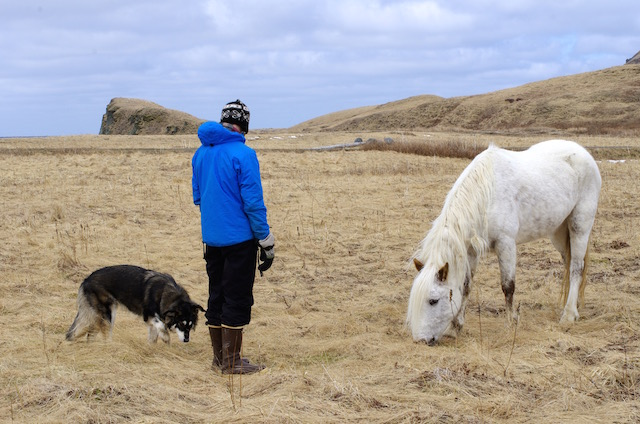
\includegraphics[scale=0.22]{../media/person}
		\hspace{0.6cm}
		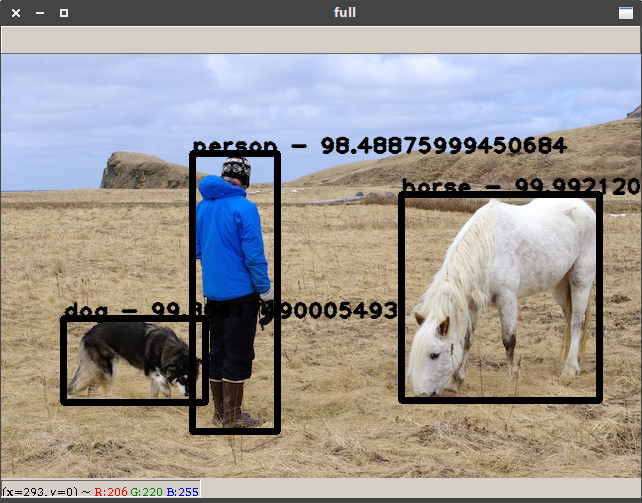
\includegraphics[scale=0.22]{Imgs/pessoa_cavalo_cao}
	\end{figure}
\end{frame}
	
	
	
\begin{frame}
	\frametitle{Teste 3}
	\begin{figure}
		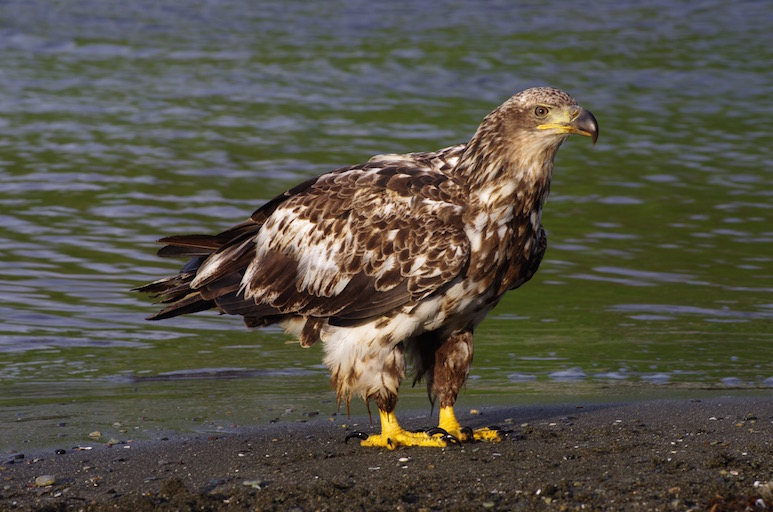
\includegraphics[scale=0.2]{../media/eagle}
		\hspace{0.6cm}
		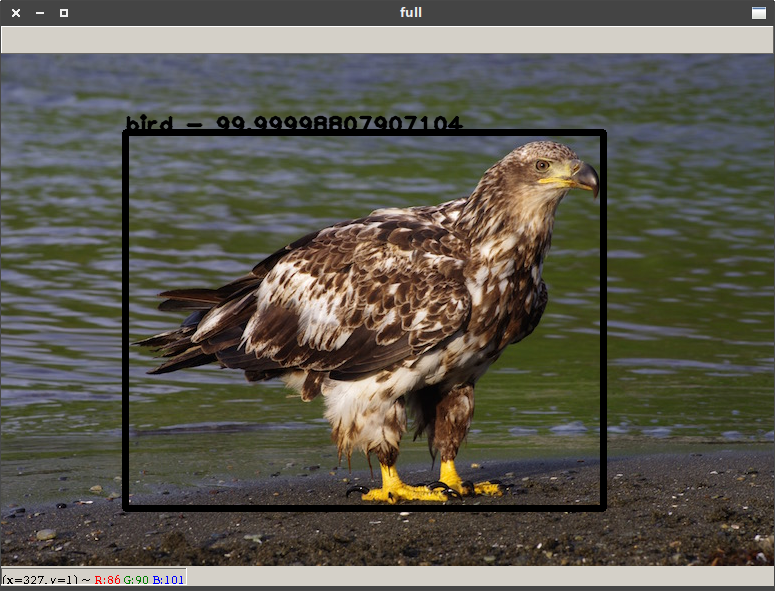
\includegraphics[scale=0.2]{Imgs/bird}
	\end{figure}

\end{frame}

	\section{Interface Web}
	\subsection{Overview}
	
	\begin{frame}
	\frametitle{Interface Web - Overview}
		Para a interface utilizou-se o framework Django.
		
		Como referências para o código apresentado foram utilizados:
		
		\vspace{1cm}
		
		\begin{itemize}
			\item Código freeCodeCamp Django Course.
			\item github.com/thalescast/PDI
			\item Código Próprio
		\end{itemize}
	\end{frame}

	
	\subsection{Resultados Web}
	\begin{frame}
	\frametitle{Resultados Web}
		O código do script pode ser integrado em um App Web:
		
	\begin{figure}
		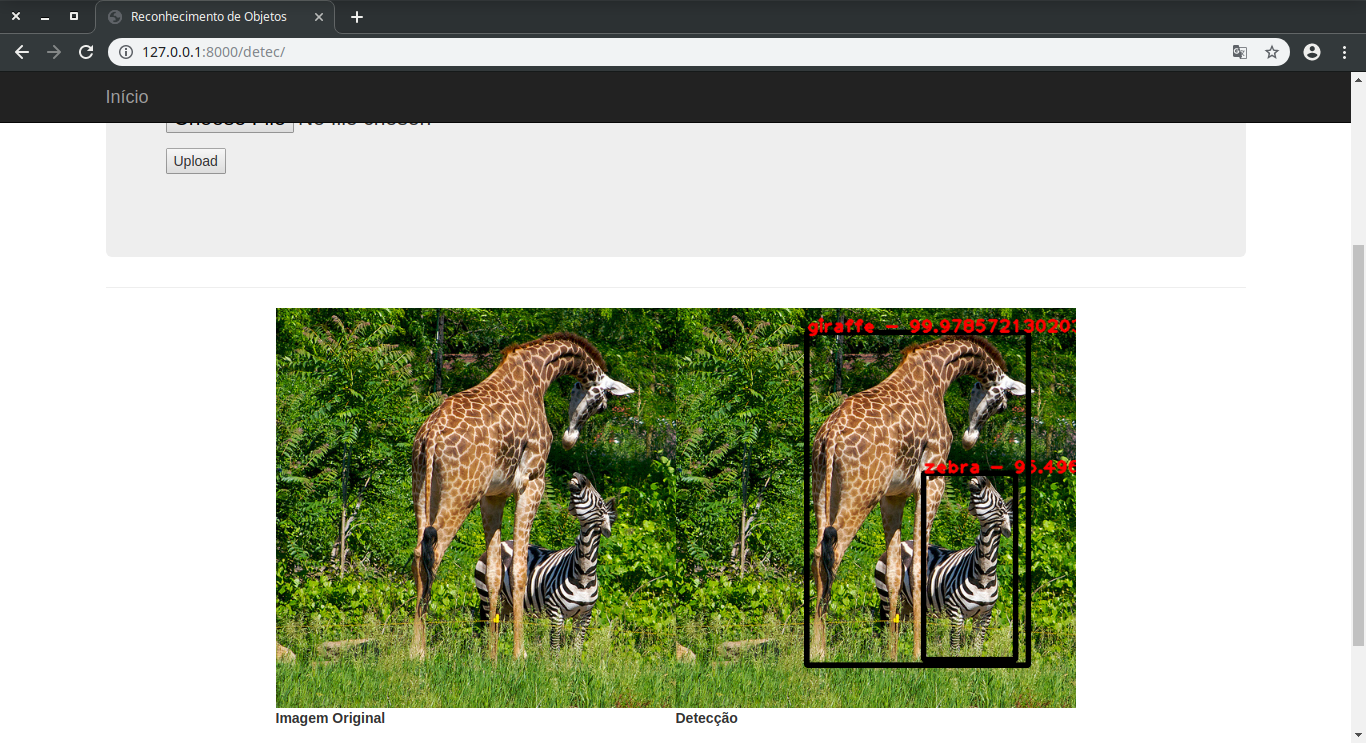
\includegraphics[scale=0.2]{Imgs/giraffe_django}
	\end{figure}
	
\end{frame}
	
	
	\begin{frame}
	\frametitle{Resultados Web}

	
	\begin{figure}
		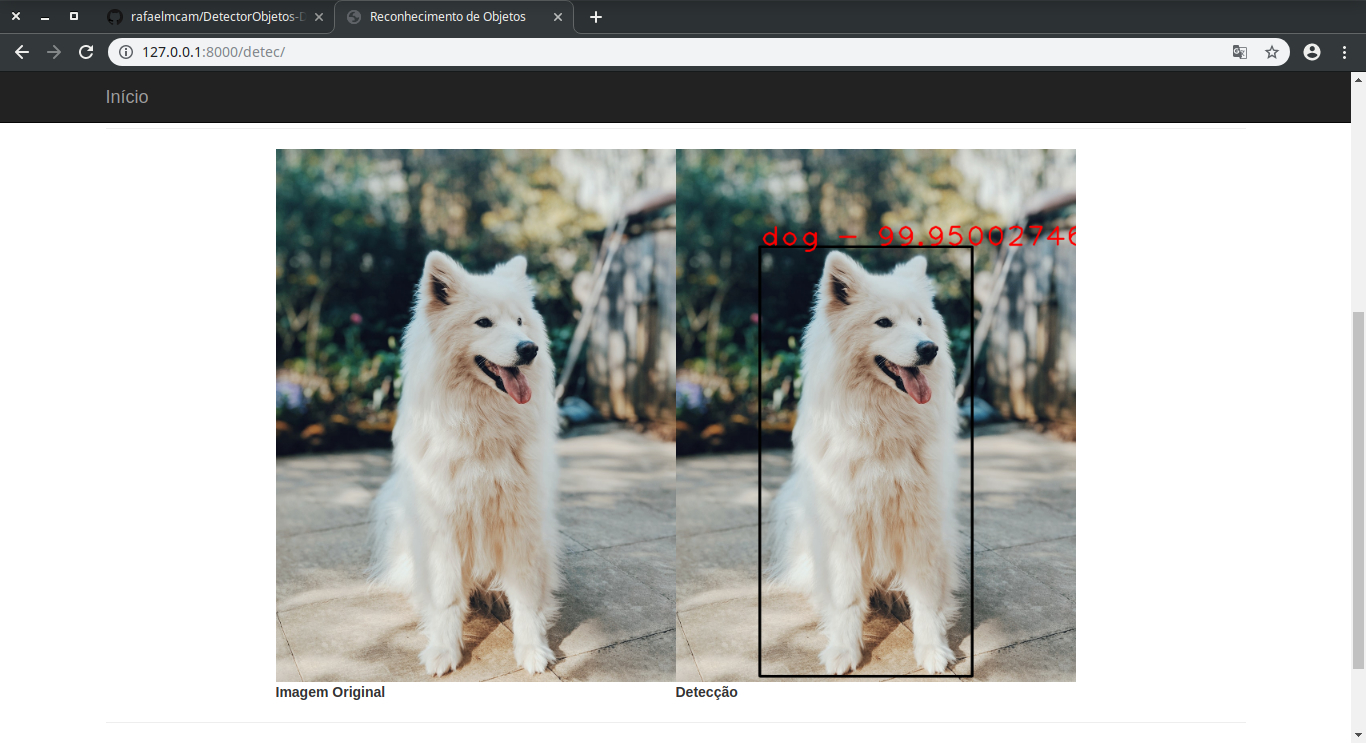
\includegraphics[scale=0.2]{Imgs/dog_django}
	\end{figure}
	
\end{frame}


\begin{frame}
	
	\begin{center}
		Código disponível neste repositório.
		
		Obrigado.
	\end{center}
	
\end{frame}
\end{document}

